%
% Copyright 2018 Joel Feldman, Andrew Rechnitzer and Elyse Yeager.
% This work is licensed under a Creative Commons Attribution-NonCommercial-ShareAlike 4.0 International License.
% https://creativecommons.org/licenses/by-nc-sa/4.0/
%
\questionheader{ex:s3.2}

%%%%%%%%%%%%%%%%%%
\subsection*{\Conceptual}
%%%%%%%%%%%%%%%%%%
\begin{question}
Write out the first five partial sums corresponding to the series
$\displaystyle\sum_{n=1}^{\infty} \frac{1}{n}$.

You don't need to simplify the terms.
\end{question}
\begin{hint}
$S_N$ is the sum of the terms corresponding to $n=1$ through $n=N$.
\end{hint}
\begin{answer}

$\begin{array}{l|l}
\mathbf{N}&\mathbf{S_N}\\
\hline
1 & 1\\[7pt]
2 & 1+\frac12\\[7pt]
3 & 1+\frac12 + \frac13\\[7pt]
4 & 1+\frac12 + \frac13+\frac14\\[7pt]
5 & 1+\frac12 + \frac13+\frac14+\frac15\\[7pt]
\end{array}$
\end{answer}
\begin{solution}
The $N$th term of the sequence of partial sums, $S_N$, is the sum of the first $N$ terms of the series $\displaystyle\sum_{n=1}^{\infty} \frac{1}{n}$.
\[\begin{array}{l|l}
\mathbf{N}&\mathbf{S_N}\\
\hline
1 & 1\\[7pt]
2 & 1+\frac12\\[7pt]
3 & 1+\frac12 + \frac13\\[7pt]
4 & 1+\frac12 + \frac13+\frac14\\[7pt]
5 & 1+\frac12 + \frac13+\frac14+\frac15\\[7pt]
\end{array}
\]\end{solution}
%%%%%%%%%%%%%%%%%%%
\begin{Mquestion}\label{prob_s3.2:cookies}
Every student who comes to class brings their instructor cookies, and leaves them on the instructor's desk. Let $C_k$ be the total number of cookies on the instructor's desk after the $k$th student comes.

If $C_{11}=20$, and $C_{10}=17$, how many cookies did the 11th student bring to class?
\end{Mquestion}
\begin{hint}
Note $C_k$ is the cumulative number of cookies.
\end{hint}
\begin{answer}
3
\end{answer}
\begin{solution}
If there were a total of 17 cookies before Student 11 came, and 20 cookies after, then Student 11 brought 3 cookies.

\begin{center}
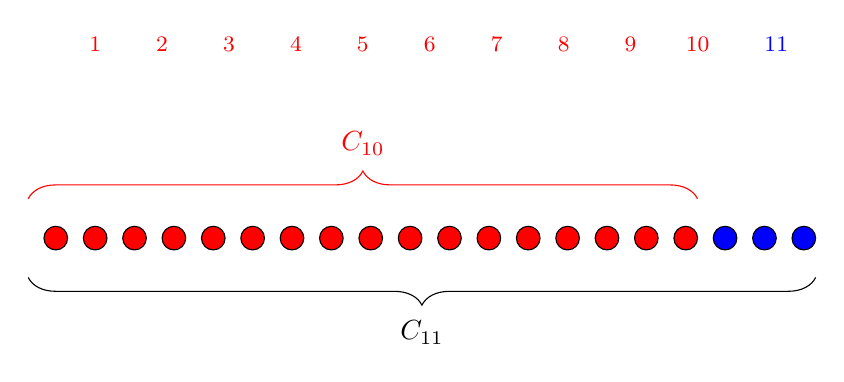
\begin{tikzpicture}
\foreach \x in {1,...,17}{
	\draw[fill=red] (\x/2,0) arc(0:360:1.5mm);}
\foreach \x in {18,19,20}{
	\draw[fill=blue] (\x/2,0) arc(0:360:1.5mm);}
\draw[red, decorate, decoration={brace, amplitude=10pt}] (0,.5)--(8.5,0.5) node[midway, yshift=7mm]{$C_{10}$};
\draw[decorate, decoration={brace, amplitude=10pt, mirror}] (0,-.5)--(10,-0.5) node[midway, yshift=-7mm]{$C_{11}$};
\begin{scope}[scale=0.5]
\color{red}
\foreach \x in {1,...,10}{
	\YEstickfig{\x*1.7}{4}{\x}
	\draw(\x*1.7,4.5) node[above]{\footnotesize $\x$};}
\color{blue}
	\YEstickfig{19}{4}{11}
	\draw(19,4.5) node[above]{\footnotesize $11$};
\end{scope}
\end{tikzpicture}
\end{center}

\end{solution}
%%%%%%%%%%%%%%%%%%%
\begin{Mquestion}\label{prob_s3.2:partsums}
Suppose the sequence of partial sums of the series $\displaystyle\sum_{n=1}^\infty a_n$
is $\{S_N\} = \left\{\dfrac{N}{N+1}\right\}$.
\begin{enumerate}[(a)]
\item What is $\{a_n\}$?
\item What is $\lim\limits_{n \to \infty} a_n $?
\item Evaluate $\displaystyle\sum_{n=1}^\infty a_n$.
\end{enumerate}
\end{Mquestion}
\begin{hint}
How is (a) related to Question~\ref{prob_s3.2:cookies}?
\end{hint}
\begin{answer}
(a) $\displaystyle a_n = \begin{cases}
\frac12 &\mbox{ if } n=1\\
\dfrac{1}{n(n+1)} &\mbox{ else }\\
\end{cases}$
\qquad\qquad (b) 0 \qquad (c) 1
\end{answer}
\begin{solution}
\begin{enumerate}[(a)]
\item We find $\{a_n\}$ from $\{S_N\}$ using the same logic as Question~\ref{prob_s3.2:cookies}. $S_N$ is the sum of the first $N$ terms of $\{a_n\}$, and $S_{N-1}$ is the sum of all the same terms \emph{except} $a_N$. So, $a_N = S_N-S_{N-1}$ when $N \geq 2$. Written another way:
\begin{align*}
\color{blue}S_N&\color{blue}=a_1+a_2+a_3+\cdots+a_{N-2}+a_{N-1}+a_N\\
\color{red}S_{N-1}&\color{red}=a_1+a_2+a_3+\cdots+a_{N-2}+a_{N-1}\\
\intertext{So,}
\color{blue}S_N
-\color{red}S_{N-1}
&=\color{blue}\Big[a_1+a_2+a_3+\cdots+a_{N-2}+a_{N-1}+a_N\Big]\\&-
\color{red}\Big[a_1+a_2+a_3+\cdots+a_{N-2}+a_{N-1}
\Big]\\
&=\color{blue}a_N
\intertext{So, we calculate}
a_N&=S_N-S_{N-1}=\left(\dfrac{N}{N+1}\right)-\left(\dfrac{N-1}{N-1+1}\right)\\
&=\frac{N^2}{N(N+1)}-\frac{N^2-1}{N(N+1)}\\
&=\frac{1}{N(N+1)}
\intertext{Therefore,}
a_n&=\frac{1}{n(n+1)}
\end{align*}
Remark: the formula given for $S_N$ has $S_0=0$, which makes sense: the sum of no terms at all should be 0. However, it is common for a sequence of partial sums to start at $N=1$. (This fits our definition of a partial sum--we don't really define the ``sum of no terms.") In this case, $a_1$ must be calculated separately from the other terms of $\{a_n\}$. To find $a_1$, we simply set $a_1=S_1$, which (to reiterate) might not be the same as $S_1-S_0$.
\item
\[\lim\limits_{n \to \infty} a_n =\lim\limits_{n \to \infty} \dfrac{1}{n(n+1)}=0.\]
That is, the terms we're adding up are getting very, very small as we go along.
\item By Definition~\eref{CLP101}{def:SRseries} in the CLP--II text,
\[\sum_{n=1}^\infty a_n = \lim_{N \to \infty}S_N = \lim_{N \to \infty}\dfrac{N}{N+1}=1\]
That is, as we add more and more terms of our series, our cumulative sum gets very, very close to 1.
\end{enumerate}
\end{solution}
%%%%%%%%%%%%%%%%%%%
\begin{question}
Suppose the sequence of partial sums of the series $\displaystyle\sum_{n=1}^\infty a_n$
is $\{S_N\} = \left\{(-1)^N+\dfrac{1}{N}\right\}$.

What is $\{a_n\}$?

\end{question}
\begin{hint}
You'll have to calculate $a_1$ separately from the other terms.
\end{hint}
\begin{answer}
 $a_n=\begin{cases}
0 & \mbox{ if } n=1\\
2(-1)^{n}  -\frac{1}{n(n-1)} &\mbox{ else}
\end{cases}$\qquad\qquad
\end{answer}
\begin{solution}
As in Question~\ref{prob_s3.2:partsums},
\begin{align*}
a_N&=S_N-S_{N-1}=\left[(-1)^N+\dfrac{1}{N}\right]-\left[(-1)^{N-1}+\dfrac{1}{N-1}\right]\\
&=(-1)^N-(-1)^{N-1} + \frac{1}{N}-\frac{1}{N-1}\\
&=(-1)^N+(-1)^{N} + \frac{N-1}{N(N-1)}-\frac{N}{N(N-1)}\\
&=2(-1)^{N}  -\frac{1}{N(N-1)}
\intertext{Note, however, that $a_N$ is only the same as $S_N-S_{N-1}$ when $N \geq 2$: otherwise, we're trying to calculate $S_1-S_0$, but $S_0$ is not defined. So, we find $a_1$ separately:}
a_1&=S_1=(-1)^1+\frac{1}{1}=0
\intertext{All together:}
a_n&=\begin{cases}
0 & \mbox{ if } n=1\\
2(-1)^{n}  -\frac{1}{n(n-1)} &\mbox{ else}
\end{cases}
\end{align*}
\end{solution}
%%%%%%%%%%%%%%%%%%%
\begin{Mquestion}
Let $f(N)$ be a formula for the $N$th partial sum of $\displaystyle\sum_{n=1}^\infty a_n$. (That is, $f(N)=S_N$.) If $f'(N)<0$ for all $N > 1$, what does that say about $a_n$?
\end{Mquestion}
\begin{hint}
When does adding a number decrease the total sum?
\end{hint}
\begin{answer}
$a_n < 0$ for all $n \geq 2$
\end{answer}
\begin{solution}
If $f'(N)<0$, that means $f(N)$ is decreasing. So, adding more terms makes for a smaller sum. That means the terms we're adding are negative. That is,
$a_n < 0$ for all $n \geq 2$.
\end{solution}

%%%%%%%%%%%%%%%%%%%


\Instructions{Questions~\ref{prob_s3.2:pic1} through \ref{prob_s3.2:pic3} invite you to explore geometric sums in a geometric way. This is complementary to than the algebraic method discussed in the text.}
%%%%%%%%%%%%%%%%%%%
\begin{question}\label{prob_s3.2:pic1}
Suppose the triangle outlined in red in the picture below has area one.
\begin{center}\begin{tikzpicture}[scale=0.5]
\foreach \x in {0,1,2}{
	\draw (0,0)+(-30+120*\x:8cm) coordinate(o\x){};}
\filldraw (o0)--(o1)--(o2)--(o0);
\foreach \y in {1,...,10}{
\SUBTRACT{3}{\y}{\w}
\POWER{2}{\w}{\l};
\SUBTRACT{4}{\y}{\z}
\POWER{2}{\z}{\t}
\SUBTRACT{8}{\t}{\h}
		\foreach \x in {0,1,2}{
			\draw (0,\h)+(30-120*\x:\l cm) coordinate(g\x\y){};
}
\filldraw[white, fill=white] (g0\y)--(g1\y)--(g2\y)--(g0\y);}
\draw[line width=5pt, red] (o0)--(o1)--(o2)--cycle;
\end{tikzpicture}
\end{center}
\begin{enumerate}[(a)]
\item Express the combined area of the black triangles as a series, assuming the pattern continues forever.
\item Evaluate the series using the picture (\emph{not} the formula from your book).
\end{enumerate}
\end{question}
\begin{hint}
For (b), imagine cutting up the triangle into its black and white parts, then sharing it equally among a certain number of friends. What is the easiest number of friends to share with, making sure each has the same area in their pile?
\end{hint}
\begin{answer}
(a) $\displaystyle\sum_{n=1}^\infty \frac{2}{4^n}$ \qquad (b) $\dfrac23$
\end{answer}
\begin{solution}
(a)
To generate the pattern, we repeat the following steps:
\begin{itemize}
\item divide the top triangle into four triangles of equal area,
\item colour the bottom two of them black, and
\item leave the middle one white.
\end{itemize}
Every time we repeat this sequence, we divide up a triangle with an area one-quarter the size of our previous triangle, and take two of the four resulting pieces. So, our area should end up as a geometric sum with common ratio $r=\dfrac14$, and coefficient $a=2$. This is shown more explicitly below.

Since the entire triangle (outlined in red) has area 1, the four smaller triangles below each have area $\dfrac14$. The two black triangles will be added to our total black area; the blue triangle will be subdivided.
\begin{center}\begin{tikzpicture}[scale=0.5]
\foreach \x in {0,1,2}{
	\draw (0,0)+(-30+120*\x:8cm) coordinate(o\x){};}
\filldraw (o0)--(o1)--(o2)--(o0);
\foreach \y in {1}{
\SUBTRACT{3}{\y}{\w}
\POWER{2}{\w}{\l};
\SUBTRACT{4}{\y}{\z}
\POWER{2}{\z}{\t}
\SUBTRACT{8}{\t}{\h}
		\foreach \x in {0,1,2}{
			\draw (0,\h)+(30-120*\x:\l cm) coordinate(g\x\y){};
}
\filldraw[white, fill=white] (g0\y)--(g1\y)--(g2\y)--(g0\y);}
\filldraw[blue, fill=blue] (g01)--(g21)--(o1)--(g01);
\draw[line width=5pt,  red] (o0)--(o1)--(o2)--cycle;
\draw[white] (-3.5,-1.5) node{$\frac{1}{4}$};
\draw[white] (3.5,-1.5) node{$\frac{1}{4}$};
\end{tikzpicture}
\end{center}

The blue triangle had area $\dfrac{1}{4}$, so each of the small black triangles below has area $\left(\dfrac14\right)\left(\dfrac14\right)=\dfrac{1}{4^2}$.

\begin{center}\begin{tikzpicture}[scale=0.5]
\foreach \x in {0,1,2}{
	\draw (0,0)+(-30+120*\x:8cm) coordinate(o\x){};}
\filldraw (o0)--(o1)--(o2)--(o0);
\foreach \y in {1,2}{
\SUBTRACT{3}{\y}{\w}
\POWER{2}{\w}{\l};
\SUBTRACT{4}{\y}{\z}
\POWER{2}{\z}{\t}
\SUBTRACT{8}{\t}{\h}
		\foreach \x in {0,1,2}{
			\draw (0,\h)+(30-120*\x:\l cm) coordinate(g\x\y){};
}
\filldraw[white, fill=white] (g0\y)--(g1\y)--(g2\y)--(g0\y);}
\filldraw[blue, fill=blue] (g02)--(g22)--(o1)--(g02);
\draw[line width=5pt,  red] (o0)--(o1)--(o2)--cycle;
\draw[white] (-3.5,-1.5) node{$\frac{1}{4}$};
\draw[white] (3.5,-1.5) node{$\frac{1}{4}$};
\draw[white] (-2,3) node{$\frac{1}{4^2}$};
\draw[white] (2,3) node{$\frac{1}{4^2}$};
\end{tikzpicture}
\end{center}
Each time we make another subdivision, we add two black triangles, each with $\dfrac{1}{4}$ the area of the previous black triangles. So, our total black area is:
\[2\left(\frac14\right)+2\left(\frac{1}{4^2}\right)+2\left(\frac{1}{4^3}\right)+2\left(\frac{1}{4^4}\right)+\cdots = \sum_{n=1}^\infty \frac{2}{4^n}\]

\noindent (b) To evalutate the series,  we imagine gathering up all our little triangles and sorting them into three identical piles: the bottom three triangles go in three different piles, the three triangles directly above them go in three different piles, etc. (In the picture below, different colours correspond to different piles.)

\begin{center}\begin{tikzpicture}[scale=0.5]
\foreach \x in {0,1,2}{
	\draw (0,0)+(-30+120*\x:8cm) coordinate(o\x){};}
\filldraw[red] (o0)--(o1)--(o2)--(o0);
\draw (o0)--(o2) coordinate[midway](b){};
\filldraw[blue] (o0)--(b)--(o1)--(o0);
\foreach \y in {1,...,10}{
\SUBTRACT{3}{\y}{\w}
\POWER{2}{\w}{\l};
\SUBTRACT{4}{\y}{\z}
\POWER{2}{\z}{\t}
\SUBTRACT{8}{\t}{\h}
		\foreach \x in {0,1,2}{
			\draw (0,\h)+(30-120*\x:\l cm) coordinate(g\x\y){};
}
\filldraw[white, fill=white] (g0\y)--(g1\y)--(g2\y)--(g0\y);}
\draw[line width=5pt,  red] (o0)--(o1)--(o2)--cycle;
\end{tikzpicture}
\end{center}

Since the piles all have equal area, each pile has a total area of $\dfrac 13$. The  black area shaded in the problem corresponds to \emph{two} piles (red and blue above), so
\[\sum_{n=1}^\infty \frac{2}{4^n}=\frac23\]
\end{solution}
%%%%%%%%%%%%%%%%%%%

\begin{Mquestion}\label{prob_s3.2:pic2}
Suppose the square outlined in red in the picture below has area one.
\begin{center}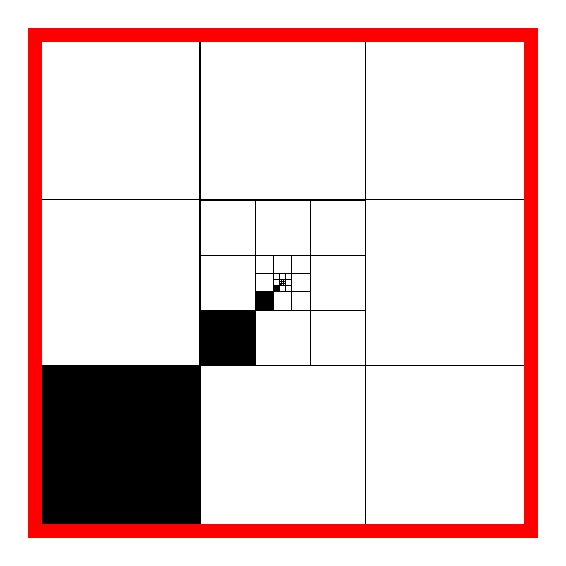
\begin{tikzpicture}[scale=0.7]
\draw (0,0) grid[step=3cm] (9,9);
\draw (3,3) grid[step=1cm] (6,6);
\draw (4,4) grid[step=0.3333cm] (5,5);
\draw (4.3333,4.3333) grid[step=0.111111cm] (4.6667,4.6667);
\draw (4.4444,4.4444) grid[step=0.037037037cm] (4.5555,4.5555);
\draw[fill] (0,0) rectangle (3,3);
\draw[fill] (3,3) rectangle (4,4);
\draw[fill] (4,4) rectangle (4.3333,4.3333);
\draw[fill] (4.3333,4.3333) rectangle (4.4444,4.4444);
\draw[fill] (4.4444,4.4444) rectangle (4.4814,4.4814);
\draw[line width=5pt,  red] (0,0) rectangle (9,9);
\end{tikzpicture}
\end{center}
\begin{enumerate}[(a)]
\item Express the combined area of the black square as a series, assuming the pattern continues forever.
\item Evaluate the series using the picture (\emph{not} the formula from your book).
\end{enumerate}
\end{Mquestion}
\begin{hint}
Compare to Question~\ref{prob_s3.2:pic1}.
\end{hint}
\begin{answer}
(a) $\displaystyle\sum_{n=1}^\infty \frac{1}{9^n}$ \qquad (b) $\dfrac{1}{8}$
\end{answer}
\begin{solution}
(a) The pattern can be described as follows: divide the innermost square into 9 equal parts (a $3\times 3$ grid), choose one square to be black, and another square to subdivide.

The area of the red (outermost) square is 1, so the area of the largest black square is $\dfrac19$. The area of the central, blue square below is also $\dfrac19$.
\begin{center}\begin{tikzpicture}[scale=0.7]
\draw (0,0) grid[step=3cm] (9,9);
\draw[fill] (0,0) rectangle (3,3);
\draw[fill=blue] (3,3) rectangle (6,6);
\draw[white] (1.5,1.5) node{$\dfrac19$};
\draw[white] (4.5,4.5) node{$\dfrac19$};
\draw[line width=5pt,  red] (0,0) rectangle (9,9);
\end{tikzpicture}
\end{center}
When we subdivide the blue square, the subdivisions each have one-ninth its area, or $\dfrac{1}{9^2}$.
\begin{center}\begin{tikzpicture}[scale=0.7]
\draw (0,0) grid[step=3cm] (9,9);
\draw (3,3) grid[step=1cm] (6,6);
\draw[fill] (0,0) rectangle (3,3);
\draw[white] (1.5,1.5) node{$\dfrac19$};
\draw[fill] (3,3) rectangle (4,4);
\draw[white] (3.5,3.5) node{\footnotesize $\dfrac1{9^2}$};
\draw[fill=blue] (4,4) rectangle (5,5);
\draw[white] (4.5,4.5) node{\footnotesize $\dfrac1{9^2}$};
\draw[line width=5pt,  red] (0,0) rectangle (9,9);
\end{tikzpicture}
\end{center}

We continue taking squares that are one-ninth the area of the previous square. So, our total black area is
\[\frac{1}{9}+\frac{1}{9^2}+\frac{1}{9^3}+\cdots = \sum_{n=1}^\infty \frac{1}{9^n}\]

(b) If we cut up this square along the marks, we can easily share it equally among 8 friends: there are eight squares of area $\dfrac19$ along the outer ring,
eight squares of area $\dfrac1{9^2}$ along the next ring in, and so on.

\begin{center}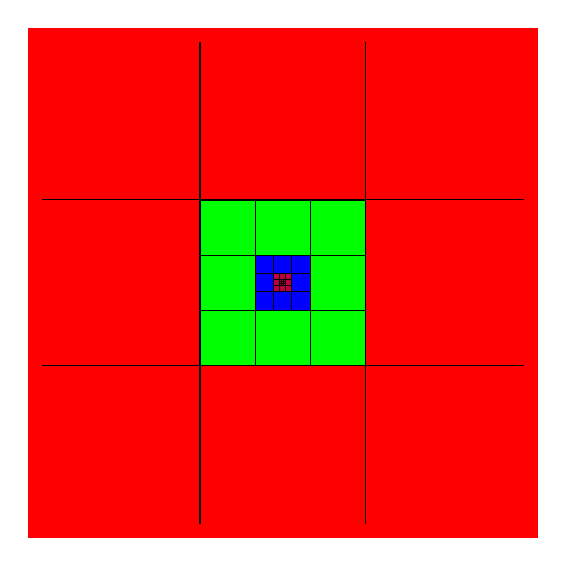
\begin{tikzpicture}[scale=0.7]
\fill[red] (0,0) rectangle (9,9);
\fill[green] (3,3) rectangle (6,6);
\fill[blue] (4,4) rectangle (5,5);
\fill[purple] (4.3333,4.3333) rectangle (4.6667,4.6667);
\draw (0,0) grid[step=3cm] (9,9);
\draw (3,3) grid[step=1cm] (6,6);
\draw (4,4) grid[step=0.3333cm] (5,5);
\draw (4.3333,4.3333) grid[step=0.111111cm] (4.6667,4.6667);
\draw (4.4444,4.4444) grid[step=0.037037037cm] (4.5555,4.5555);
\draw[line width=5pt, red] (0,0) rectangle (9,9);
\end{tikzpicture}
\end{center}

Since the eight friends all get the same total area, the area each friend gets is $\dfrac{1}{8}$. The area shaded in black in the question corresponds to the pile given to one friend. So,
\[\sum_{n=1}^\infty \frac{1}{9^n}=\frac18\]
\end{solution}
%%%%%%%%%%%%%%%%%%%


\begin{Mquestion}\label{prob_s3.2:pic3}
In the style of Questions~\ref{prob_s3.2:pic1} and \ref{prob_s3.2:pic2}, draw a picture that represents
$\displaystyle\sum_{n=1}^{\infty}\frac{1}{3^n}$
as an area.
\end{Mquestion}
\begin{hint}
Iteratively divide a shape into thirds.
\end{hint}
\begin{answer}
Two possible pictures:
\begin{center}
\begin{tikzpicture}
\draw[red, thick] (0,0) rectangle (9,5);
\foreach \a in {1,...,5}{
	\POWER{3}{\a}{\pow}
	\SUBTRACT{\pow}{1}{\num}
	\MULTIPLY{2}{\pow}{\den}
	\DIVIDE{\num}{\den}{\Sa}
	\MULTIPLY{9}{\Sa}{\left}
	\SUBTRACT{9}{\left}{\right}
	\filldraw[fill opacity=0.2] (\left,0) rectangle (0,5);
	\draw (\right,0)--(\right,5);
	}
\end{tikzpicture}

\begin{tikzpicture}[scale=0.8]
\draw[red, thick] (0,0) rectangle (9,9);
\foreach \a in {1,...,4}{
	\POWER{3}{\a}{\pow}
	\SUBTRACT{\pow}{1}{\num}
	\MULTIPLY{2}{\pow}{\den}
	\DIVIDE{\num}{\den}{\Sa}
	\MULTIPLY{9}{\Sa}{\left}
	\SUBTRACT{9}{\left}{\right}
	\SUBTRACT{\right}{\left}{\dx}
	\MULTIPLY{\dx}{3}{\dy}
	\filldraw[fill opacity={1-\a/5}] (\left,4.5-\dy/2) rectangle (\left-\dx,4.5+\dy/2);
	\draw (\right,4.5-\dy/2)--(\right,4.5+\dy/2);
	\filldraw[fill opacity={1-\a/5}] (\left,4.5-\dy/2) rectangle (\left+\dx,4.5-\dy/2+\dx);
	\draw (\left,4.5+\dy/2-\dx)--(\right,4.5+\dy/2-\dx);
	}
\end{tikzpicture}
\end{center}
\end{answer}
\begin{solution}

If we start with a shape of area 1, and iteratively divide it into thirds, taking one of the three newly created pieces each time, then the area we take will be equal to the desired series, $\displaystyle\sum_{n=1}^\infty \frac{1}{3^n}$.

One way to do this is to start with a rectangle, make three vertical strips, then keep the left strip and subdivide the middle strip.

\begin{center}
\begin{tikzpicture}[scale=0.5]
\draw[red, thick] (0,0) rectangle (9,5);
\foreach \a in {1}{
	\POWER{3}{\a}{\pow}
	\SUBTRACT{\pow}{1}{\num}
	\MULTIPLY{2}{\pow}{\den}
	\DIVIDE{\num}{\den}{\Sa}
	\MULTIPLY{9}{\Sa}{\left}
	\SUBTRACT{9}{\left}{\right}
	\filldraw[fill opacity=0.2] (\left,0) rectangle (0,5);
	\draw (\right,0)--(\right,5);
	}
\draw[thick, ->, red] (10,2.5)--(11,2.5);
\begin{scope}[xshift=12cm]
\draw[red, thick] (0,0) rectangle (9,5);
\foreach \a in {1,2}{
	\POWER{3}{\a}{\pow}
	\SUBTRACT{\pow}{1}{\num}
	\MULTIPLY{2}{\pow}{\den}
	\DIVIDE{\num}{\den}{\Sa}
	\MULTIPLY{9}{\Sa}{\left}
	\SUBTRACT{9}{\left}{\right}
	\filldraw[fill opacity=0.2] (\left,0) rectangle (0,5);
	\draw (\right,0)--(\right,5);
	}
\end{scope}
\end{tikzpicture}

\begin{tikzpicture}[scale=0.5]
\draw[thick, ->, red] (-2,2.5)--(-1,2.5);
\draw[red, thick] (0,0) rectangle (9,5);
\foreach \a in {1,...,3}{
	\POWER{3}{\a}{\pow}
	\SUBTRACT{\pow}{1}{\num}
	\MULTIPLY{2}{\pow}{\den}
	\DIVIDE{\num}{\den}{\Sa}
	\MULTIPLY{9}{\Sa}{\left}
	\SUBTRACT{9}{\left}{\right}
	\filldraw[fill opacity=0.2] (\left,0) rectangle (0,5);
	\draw (\right,0)--(\right,5);
	}
\draw[thick, ->, red] (10,2.5)--(11,2.5);
\begin{scope}[xshift=12cm]
\draw[red, thick] (0,0) rectangle (9,5);
\foreach \a in {1,2,3,4}{
	\POWER{3}{\a}{\pow}
	\SUBTRACT{\pow}{1}{\num}
	\MULTIPLY{2}{\pow}{\den}
	\DIVIDE{\num}{\den}{\Sa}
	\MULTIPLY{9}{\Sa}{\left}
	\SUBTRACT{9}{\left}{\right}
	\filldraw[fill opacity=0.2] (\left,0) rectangle (0,5);
	\draw (\right,0)--(\right,5);
	}
\end{scope}
\end{tikzpicture}
\end{center}

We see that the total area we take approaches one-half the total area of the figure, so
$\displaystyle\sum_{n=1}^\infty \frac{1}{3^n} = \frac12$.

Alternately, instead of always taking vertical strips, we could alternate vertical and horizontal slices.
\begin{center}

\begin{tikzpicture}[scale=0.5]
\draw[red, thick] (0,0) rectangle (9,9);
\foreach \a in {1}{
	\POWER{3}{\a}{\pow}
	\SUBTRACT{\pow}{1}{\num}
	\MULTIPLY{2}{\pow}{\den}
	\DIVIDE{\num}{\den}{\Sa}
	\MULTIPLY{9}{\Sa}{\left}
	\SUBTRACT{9}{\left}{\right}
	\SUBTRACT{\right}{\left}{\dx}
	\MULTIPLY{\dx}{3}{\dy}
	\filldraw[fill opacity={1-\a/5}] (\left,4.5-\dy/2) rectangle (\left-\dx,4.5+\dy/2);
	\draw (\right,4.5-\dy/2)--(\right,4.5+\dy/2);
	}
\draw[thick, ->, red] (10,4.5)--(11,4.5);
\begin{scope}[xshift=12cm]
\draw[red, thick] (0,0) rectangle (9,9);
\foreach \a in {1}{
	\POWER{3}{\a}{\pow}
	\SUBTRACT{\pow}{1}{\num}
	\MULTIPLY{2}{\pow}{\den}
	\DIVIDE{\num}{\den}{\Sa}
	\MULTIPLY{9}{\Sa}{\left}
	\SUBTRACT{9}{\left}{\right}
	\SUBTRACT{\right}{\left}{\dx}
	\MULTIPLY{\dx}{3}{\dy}
	\filldraw[fill opacity={1-\a/5}] (\left,4.5-\dy/2) rectangle (\left-\dx,4.5+\dy/2);
	\draw (\right,4.5-\dy/2)--(\right,4.5+\dy/2);
	\filldraw[fill opacity={1-\a/5}] (\left,4.5-\dy/2) rectangle (\left+\dx,4.5-\dy/2+\dx);
	\draw (\left,4.5+\dy/2-\dx)--(\right,4.5+\dy/2-\dx);
	}
\end{scope}
\end{tikzpicture}

\begin{tikzpicture}[scale=0.5]
\draw[thick, ->, red] (-2,4.5)--(-1,4.5);
\draw[red, thick] (0,0) rectangle (9,9);
\foreach \a in {1,2}{
	\POWER{3}{\a}{\pow}
	\SUBTRACT{\pow}{1}{\num}
	\MULTIPLY{2}{\pow}{\den}
	\DIVIDE{\num}{\den}{\Sa}
	\MULTIPLY{9}{\Sa}{\left}
	\SUBTRACT{9}{\left}{\right}
	\SUBTRACT{\right}{\left}{\dx}
	\MULTIPLY{\dx}{3}{\dy}
	\filldraw[fill opacity={1-\a/5}] (\left,4.5-\dy/2) rectangle (\left-\dx,4.5+\dy/2);
	\draw (\right,4.5-\dy/2)--(\right,4.5+\dy/2);
	\filldraw[fill opacity={1-\a/5}] (\left,4.5-\dy/2) rectangle (\left+\dx,4.5-\dy/2+\dx);
	\draw (\left,4.5+\dy/2-\dx)--(\right,4.5+\dy/2-\dx);
	}

\draw[thick, ->, red] (10,4.5)--(11,4.5);
\begin{scope}[xshift=12cm]
\draw[red, thick] (0,0) rectangle (9,9);
\foreach \a in {1,2,3}{
	\POWER{3}{\a}{\pow}
	\SUBTRACT{\pow}{1}{\num}
	\MULTIPLY{2}{\pow}{\den}
	\DIVIDE{\num}{\den}{\Sa}
	\MULTIPLY{9}{\Sa}{\left}
	\SUBTRACT{9}{\left}{\right}
	\SUBTRACT{\right}{\left}{\dx}
	\MULTIPLY{\dx}{3}{\dy}
	\filldraw[fill opacity={1-\a/5}] (\left,4.5-\dy/2) rectangle (\left-\dx,4.5+\dy/2);
	\draw (\right,4.5-\dy/2)--(\right,4.5+\dy/2);
	\filldraw[fill opacity={1-\a/5}] (\left,4.5-\dy/2) rectangle (\left+\dx,4.5-\dy/2+\dx);
	\draw (\left,4.5+\dy/2-\dx)--(\right,4.5+\dy/2-\dx);
	}
\end{scope}
\end{tikzpicture}
\end{center}

In this setup, we notice that our strips come in pairs: two large vertical strips, two smaller horizontal strips, two smaller vertical strips, etc. We shaed exactly one of each, so the shaded area is one-half the total area: $\displaystyle\sum_{n=1}^\infty \frac{1}{3^n} = \frac12$.

Other solutions are possible, as well.
\end{solution}
%%%%%%%%%%%%%%%%%%%



\begin{question}
Evaluate $\displaystyle\sum_{n=0}^{100}\frac{1}{5^n}$.
\end{question}
\begin{hint}
Equation~\eref{CLP101}{eq:partialgeomsum} in the CLP--II text tells us
$\displaystyle\sum_{n=0}^N ar^n = a\dfrac{1-r^{N+1}}{1-r}$, for $r \neq 1$.
\end{hint}
\begin{answer}
$\dfrac{5^{101}-1}{4\cdot 5^{100}}$
\end{answer}
\begin{solution}
Equation~\eref{CLP101}{eq:partialgeomsum} in the CLP--II text tells us
$\displaystyle\sum_{n=0}^N ar^n = a\dfrac{1-r^{N+1}}{1-r}$, for $r \neq 1$.
Our geometric sum has $a=1$, $r=\frac{1}{5}$, and $N=100$. So:
\[\displaystyle\sum_{n=0}^{100}\frac{1}{5^n} =
\frac{1-\frac{1}{5^{101}}}{1-\frac{1}{5}} = \dfrac{5^{101}-1}{4\cdot 5^{100}}\]
\end{solution}

%%%%%%%%%%%%%%%%%%%
\begin{Mquestion}\label{prob_s3.2:cookies2}
Every student who comes to class brings their instructor cookies, and leaves them on the instructor's desk. Let $C_k$ be the total number of cookies on the instructor's desk after the $k$th student comes.

If $C_{20}=53$, and $C_{10}=17$, what does $C_{20}-C_{10}=36$ represent?
\end{Mquestion}
\begin{hint}
Note $C_k$ is the cumulative number of cookies.
\end{hint}
\begin{answer}
All together, there were 36 cookies brought by Student 11 through Student 20.
\end{answer}
\begin{solution}
After twenty students have brought their cookies, the pile numbers 53 cookies. 17 of these cookies were brought by students one through ten. So, the remainder ($53-17=36$) is the number of cookies brought by students 11, 12, 13, 14, 15, 16, 17, 18, 19, and 20, together.

\begin{center}
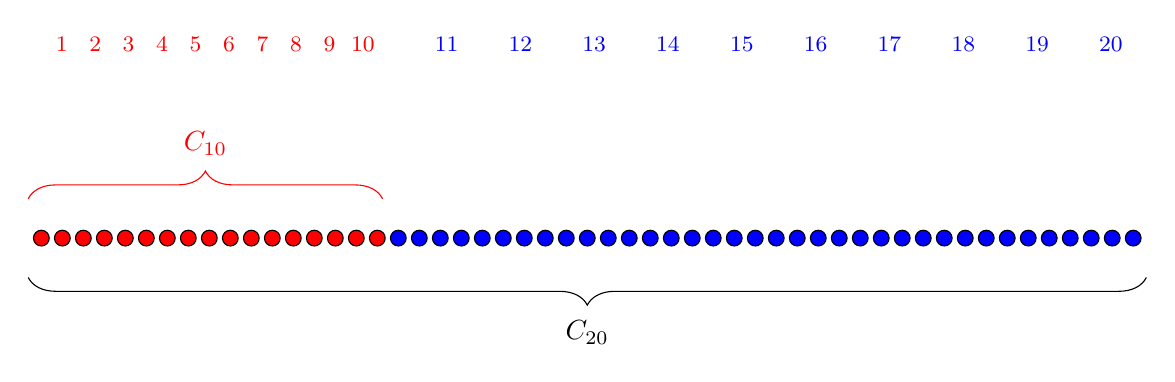
\begin{tikzpicture}
\foreach \x in {1,...,17}{
	\draw[fill=red] (\x/3.75,0) arc(0:360:1mm);}
\foreach \x in {18,...,53}{
	\draw[fill=blue] (\x/3.75,0) arc(0:360:1mm);}
\draw[red, decorate, decoration={brace, amplitude=10pt}] (0,.5)--(4.5,0.5) node[midway, yshift=7mm]{$C_{10}$};
\draw[decorate, decoration={brace, amplitude=10pt, mirror}] (0,-.5)--(14.2,-0.5) node[midway, yshift=-7mm]{$C_{20}$};
\begin{scope}[scale=0.25]
\color{red}
\foreach \x in {1,...,10}{
	\YEstickfig{\x*1.7}{8}{\x}
	\draw(\x*1.7,9) node[above]{\footnotesize $\x$};}
\color{blue}
\foreach \x in {11,...,20}{
	\YEstickfig{\x*3.75-20}{8}{\x}
	\draw(\x*3.75-20,9) node[above]{\footnotesize $\x$};}
\end{scope}

\end{tikzpicture}
\end{center}
\end{solution}

%%%%%%%%%%%%%%%%%%%
\begin{Mquestion}
Evaluate $\displaystyle\sum_{n=50}^{100}\frac{1}{5^n}$. (Note the starting index.)
\end{Mquestion}
\begin{hint}
To adjust the starting index, either factor out the first term in the series, or subtract two series. For the subtraction option, consider Question~\ref{prob_s3.2:cookies2}.
\end{hint}
\begin{answer}
$\dfrac{5^{51}-1}{4\cdot 5^{100}}$
\end{answer}
\begin{solution}
\begin{description}
\item[Solution 1:] Using the ideas of Question~\ref{prob_s3.2:cookies2}, we see:
\begin{align*}
\sum_{n={50}}^{100} \frac{1}{5^n}&=\sum_{n=0}^{100}\frac{1}{5^n}-\sum_{n=0}^{49}\frac{1}{5^n}
\intertext{That is, we want start with the sum of all the terms up to $\dfrac{1}{5^{100}}$, and then subtract off the ones we actually don't want, which is everything up to $\dfrac{1}{5^{49}}$. Now, both series are in a form appropriate for Equation~\eref{CLP101}{eq:partialgeomsum}
 in the CLP--II text.}
\sum_{n=0}^{100}\frac{1}{5^n}-\sum_{n=0}^{49}\frac{1}{5^n}&=\frac{1-\frac{1}{5^{101}}}{1-\frac15}-\frac{1-\frac{1}{5^{50}}}{1-\frac15}\\
&=\frac{5^{101}-1}{4\cdot 5^{100}}-\frac{5^{50}-1}{4\cdot 5^{49}}\left(\frac{5^{51}}{5^{51}}\right)\\
&=\frac{5^{101}-1}{4\cdot 5^{100}}-\frac{5^{101}-5^{51}}{4\cdot 5^{100}}\\
&=\frac{5^{51}-1}{4\cdot 5^{100}}
\end{align*}
\item[Solution 2:]
If we write out the first few terms of our series, we see we can factor out a constant to change the starting index.
\begin{align*}
\sum_{n={50}}^{100} \frac{1}{5^n}&= \frac{1}{5^{50}}+
\frac{1}{5^{51}}+\frac{1}{5^{52}}+\frac{1}{5^{53}}+\cdots +\frac{1}{5^{100}}\\
&=\frac{1}{5^{50}}\left(\frac{1}{5^0}+\frac{1}{5^1}+\frac{1}{5^2}+\frac{1}{5^3}+\cdots +\frac{1}{5^{50}}\right)\\
&=\sum_{n=0}^{50}\frac{1}{5^{50}}\cdot\frac{1}{5^n}
\intertext{Now, our sum is in the form of Equation~\eref{CLP101}{eq:partialgeomsum}
 in the CLP--II text
with $a=\dfrac{1}{5^{50}},$ $r=\dfrac15$, and $N=50$.}
\sum_{n=0}^{50}\frac{1}{5^{50}}\cdot\frac{1}{5^n}&=\frac{1}{5^{50}}\cdot\frac{1-\frac{1}{5^{51}}}{1-\frac15}=\frac{1-\frac{1}{5^{51}}}{4\cdot 5^{49}}\left(\frac{5^{51}}{5^{51}}\right)\\
&=\frac{5^{51}-1}{4\cdot 5^{100}}
\end{align*}
\end{description}
\end{solution}
%%%%%%%%%%%%%%%%%%%
%%%%%%%%
\begin{question}
\begin{enumerate}[(a)]
\item Starting on day $d=1$, every day you give your friend \$$\frac{1}{d+1}$, and they give \$$\frac{1}{d}$ back to you.  After a long time, how much money have you gained by this arrangement?
\item Evaluate $\displaystyle\sum_{d=1}^\infty \left(\frac{1}{d}-\frac{1}{(d+1)}\right)$.
\item Starting on day $d=1$, every day your friend gives you \$$(d+1)$, and they take \$$(d+2)$ from you.  After a long time, how much money have you gained by this arrangement?
\item Evaluate $\displaystyle\sum_{d=1}^\infty \left((d+1)-(d+2)\right)$.
\end{enumerate}
\end{question}
\begin{hint}
Express your gains in (a) and (c) as series.
\end{hint}
\begin{answer}
(a) As time passes, your gains increase, approaching \$1.
\qquad (b) 1\\
(c) As time passes, you \emph{lose} more and more money, without bound.\qquad
(d) $-\infty$
\end{answer}
\begin{solution}
(a) The table below is a record of our account, with black entries representing the money your friend gives you, and red entries representing the money you give them (which is why the red entries are negative).
\[\begin{array}{c||c|c||c}
\mathbf{d}&\color{red}\mathbf{-\frac{1}{d+1}}&\mathbf{\frac1d}&\parbox{2.5cm}{\textbf{total after day $d$}}\\[7pt]
\hline
1 & \color{red} -\frac{1}{2} & 1 & \frac{1}{2}\\[7pt]
2&\color{red}-\frac{1}{3} & \frac{1}{2}&\frac{2}{3}\\[7pt]
3&\color{red}-\frac{1}{4} & \frac{1}{3}&\frac{3}{4}\\[7pt]
4&\color{red}-\frac{1}{5} & \frac{1}{4}&\frac{4}{5}\\[7pt]
5&\color{red}-\frac{1}{6} & \frac{1}{5}&\frac{5}{6}\\[7pt]
6&\color{red}-\frac{1}{7} & \frac{1}{6}&\frac{6}{7}
\end{array}\]
After the exchange of day $n$, the amount you're left with is $\$\left(1-\frac{1}{n+1}\right)$. We see this by the cancellation in the table: the \$$\frac12$ you gave your friend on day 1 was returned on day 2; the  \$$\frac13$ you gave your friend on day 2 was returned on day 3, etc.

So, after a long time, you'll have gained close to (but always slightly less than) one dollar.

(b) The series $\displaystyle\sum_{d=1}^\infty \left(\frac{1}{d}-\frac{1}{(d+1)}\right)$ describes the scenario in (a), so by our reasoning there,
\[\displaystyle\sum_{d=1}^\infty \left(\frac{1}{d}-\frac{1}{(d+1)}\right) = \lim_{n \to \infty}\left(1-\frac{1}{n+1}\right)=1\]

(c) Again, let's set up an account book.

\[\begin{array}{c||c|c||c}
\mathbf{d}&\mathbf{d+1}&\color{red}\mathbf{-(d+2)}&\textbf{total}\\[7pt]
\hline
1 & 2& \color{red} -3 & -1\\[7pt]
2 & 3& \color{red} -4 & -2\\[7pt]
3 & 4& \color{red} -5 & -3\\[7pt]
4 & 5& \color{red} -6 & -4\\[7pt]
5 & 6& \color{red} -7 & -5\\[7pt]
6 & 7& \color{red} -8 & -6\\[7pt]
\end{array}\]
By day $d$, you've \emph{lost} \$ $d$ to your so-called friend. As time goes on, you lose more and more.

(d) The series $\displaystyle\sum_{d=1}^\infty ((d+1)-(d+2))$ exactly describes the scenario in part (c), so it diverges to $-\infty$. You can also see this by writing
$\displaystyle\sum_{d=1}^\infty ((d+1)-(d+2)) =\sum_{d=1}^\infty (-1)=-1-1-1-1-1-\cdots$.

Be careful to avoid a common mistake with telescoping series: if we look back at our account book, we see that every negative term will cancel with a positive term, with the initial $+2$ as the only term that never cancels. Your friend takes \$3, which they return the next day; then they take \$4, which they return the next day; then they take \$5, which they return the next day, and so on. It's extremely tempting to say that the series adds up to \$2, since every other term cancels out eventually. This is where we lean on Definition~\eref{CLP101}{def:SRseries} in the CLP--II text:
we evaluate the \emph{partial sums}, which always leave your friend's last withdrawal unreturned. This definition makes sense: saying ``I gained two bucks from this exchange" doesn't really capture the reality of your increasing debt.
\end{solution}

%%%%%%%%%%%%%%%
\begin{question}
Suppose $\displaystyle\sum_{n=1}^\infty a_n = A$,\quad
$\displaystyle\sum_{n=1}^\infty b_n = B$, \quad and \quad
$\displaystyle\sum_{n=1}^\infty c_n = C$.

Evaluate $\displaystyle\sum_{n=1}^\infty\left( a_n+b_n+c_{n+1}\right)$.
\end{question}
\begin{hint}
To find the difference between $\displaystyle\sum_{n=1}^\infty c_n$ and
$\displaystyle\sum_{n=1}^\infty c_{n+1}$, try writing out the first few terms.
\end{hint}
\begin{answer}
$A+B+C-c_1$
\end{answer}
\begin{solution}
Using arithmetic of series, Theorem~\eref{CLP101}{thm:SRseriesarith} in the CLP--II text, we see
\[\sum_{n=1}^\infty\left( a_n+b_n+c_{n+1}\right) = A+B+\sum_{n=1}^\infty c_{n+1}\]
The question remaining is what do to with the last series. If we write out the terms, we see the difference between $\displaystyle\sum_{n=1}^\infty c_n$ and
$\displaystyle\sum_{n=1}^\infty c_{n+1}$ is simply that the latter is missing $c_1$:
\begin{align*}
\sum_{n=1}^\infty c_{n+1}&=c_2+c_3+c_4+c_5+\cdots\\
&=\textcolor{red}{-c_1+c_1}+c_2+c_3+c_4+c_5+\cdots\\
&=\textcolor{red}{-c_1}+\sum_{n=1}^\infty c_{n}
\intertext{So,}
\sum_{n=1}^\infty\left( a_n+b_n+c_{n+1}\right)&=A+B+C-\textcolor{red}{c_1}
\end{align*}
\end{solution}
%%%%%%%%%%%%%%%%%%%
\begin{Mquestion}
Suppose $\displaystyle\sum_{n=1}^\infty a_n = A$,\quad
$\displaystyle\sum_{n=1}^\infty b_n = B \neq 0$, \quad and \quad
$\displaystyle\sum_{n=1}^\infty c_n = C$.

True or false: \textcolor{blue}{$\displaystyle\sum_{n=1}^\infty\left(\dfrac{ a_n}{b_n}+c_{n}\right) = \frac{A}{B}+C$}.
\end{Mquestion}
\begin{hint}
You might want to first consider a simpler true or false: \textcolor{blue}{$\displaystyle\sum_{n=1}^\infty \dfrac{ a_n}{b_n} \stackrel{?}{=} \dfrac{A}{B}$}.
\end{hint}
\begin{answer}
in general, false
\end{answer}
\begin{solution}
Theorem~\eref{CLP101}{thm:SRseriesarith} in the CLP--II text, arithmetic of series, doesn't mention division, because in general it doesn't work the way the question suggests. For example, let $\{a_n\}=\{b_n\} = \frac{1}{2^n}$. Then:
\begin{itemize}
\item $\sum_{n=0}^{\infty} a_n = \sum_{n=0}^\infty b_n = \frac{1}{1-\frac12}=2$, while
\item $\sum_{n=0}^{\infty}\dfrac{a_n}{b_n} = \sum_{n=0}^{\infty}1 =\infty $.
\end{itemize}
For the  statement in the question, we can take $\{a_n\}=\{b_n\} = \frac{1}{2^n}$, $A=B=2$, $\{c_n\}=\{0,0,0,\ldots\}$, and $C=0$. We see the statement is false in this case.

So, in general, the statement given is false.
\end{solution}
%%%%%%%%%%%%%%%%%%%


%%%%%%%%%%%%%%%%%%
\subsection*{\Procedural}
%%%%%%%%%%%%%%%%%%


\begin{question}[2016Q5]
To what value does the series
$\displaystyle 1 + \frac{1}{3} + \frac{1}{9} + \frac{1}{27}+ \frac{1}{81}+ \frac{1}{243} + \cdots$ converge?
\end{question}

\begin{hint}
What kind of a series is this?
\end{hint}

\begin{answer}
$ \dfrac{3}{2}$
\end{answer}

\begin{solution}
We recognize that this is a geometric series:
 \begin{align*}
 1 + \frac{1}{3} + \frac{1}{9} + \frac{1}{27}+ \frac{1}{81}+ \frac{1}{243} + \cdots&=\frac{1}{3^0}+\frac{1}{3^1}+\frac{1}{3^2}+\frac{1}{3^3}+\frac{1}{3^4}+\frac{1}{3^5}+\cdot\\
 &=\sum_{n=0}^\infty \frac{1}{3^n}
 \intertext{Using Equation~\eref{CLP101}{eq:geomsum} in the CLP--II text with $r=\dfrac13$ and $a=1$,}
 &=\frac{1}{1-\frac13}=\frac{3}{2}.
 \end{align*}
\end{solution}
%%%%%%%%%%%%%%%%%%%%


\begin{Mquestion}[M105 2015A]
Evaluate
$\displaystyle \sum_{k=7}^{\infty} \frac{1}{8^k}$
\end{Mquestion}

\begin{hint}
This is a special kind of series, that you should recognize.
\end{hint}

\begin{answer}
$ \dfrac{1}{7\times 8^6}$
\end{answer}

\begin{solution}
This is a geometric series, with ratio $r=\dfrac18$. However, it doesn't start at $k=0$, which is what we're used to.
\begin{description}
\item[Solution 1:] We write out the first few terms of the series to figure out a convenient constant to factor out.
\begin{align*}
\sum_{k=7}^{\infty} \frac{1}{8^k}&=\frac{1}{8^7}+\frac{1}{8^8}+\frac{1}{8^9}+\cdots\\
&=\frac{1}{8^7}\left(\frac{1}{8^0}+\frac{1}{8^1}+\frac{1}{8^2}+\cdots\right)\\
&=\sum_{k=0}^\infty \frac{1}{8^7}\cdot \frac{1}{8^n}
\intertext{We now evaluate the series using Equation~\eref{CLP101}{eq:geomsum}
 in the CLP--II text  with $r=\dfrac18$, $a=\dfrac{1}{8^7}$.}
&=\frac{1}{8^7}\cdot\dfrac{1}{1-\frac18} = \dfrac{1}{7\times 8^6}
\end{align*}
\item[Solution 2:] Using the idea of Question~\ref{prob_s3.2:cookies2}, we express the series we're interested in as the difference of two series that we can easily evaluate.
\begin{align*}
 \sum_{k=7}^{\infty} \frac{1}{8^k}&= \sum_{k=0}^{\infty} \frac{1}{8^k}- \sum_{k=0}^{6} \frac{1}{8^k}
 \intertext{Using Equations~\eref{CLP101}{eq:geomsum} and \eref{CLP101}{eq:partialgeomsum} in the CLP--II text,}
 &=\frac{1}{1-\frac18}-\frac{1-\frac{1}{8^7}}{1-\frac18}\\
 &=\frac{1}{7\times 8^6}
\end{align*}
\end{description}
\end{solution}

%%%%%%%%%%%%%%%%%
\begin{question}[2016Q5]
Show that the series
$\displaystyle \sum_{k=1}^{\infty} \bigg( \frac{6}{k^2} - \frac{6}{(k+1)^2} \bigg)$
converges and find its limit.
\end{question}

\begin{hint}
When you see $\displaystyle\sum_k \Big(\cdots \textcolor{red}{k}\cdots \ \ -\ \ \cdots \textcolor{red}{k+1}\cdots\Big)$,
you should  think ``telescoping series."
\end{hint}

\begin{answer}
$6$
\end{answer}

\begin{solution}
We recognize this as a telescoping series.

\[\begin{array}{c||cc||r}
\mathbf{k}&\mathbf{\frac{6}{k^2}}&\mathbf{-\frac{6}{(k+1)^2}}&\mathbf{s_k}\\
\hline
1&6&\color{red}-\frac{6}{4}&6-\color{red}\frac64\\[7pt]
2&\color{red}\frac{6}{4}&\color{orange}-\frac{6}{9}&6-\color{orange}\frac69\\[7pt]
3&\color{orange}\frac{6}{9}&\color{green}-\frac{6}{16}&6-\color{green}\frac{6}{16}\\[7pt]
4&\color{green}\frac{6}{16}&\color{blue}-\frac{6}{25}&6-\color{blue}\frac{6}{25}\\[7pt]
5&\color{blue}\frac{6}{25}&\color{purple}-\frac{6}{36}&6-\color{purple}\frac{6}{36}\\[7pt]
6&\color{purple}\frac{6}{36}&-\frac{6}{47}&6-\frac{6}{47}\\[7pt]
\vdots&&&
\end{array}\]

When we compute  the $n^{\rm th}$
partial sum, i.e. the sum of of the first $n$ terms, successive terms cancel and only
the first half of the first term, $\Big( \frac{6}{k^2} - \frac{6}{(k+1)^2} \Big)\Big|_{k=1}$,
and the second half of the $n^{\rm th}$ term,
$\Big( \frac{6}{k^2} - \frac{6}{(k+1)^2} \Big)\Big|_{k=n}$, survive. That is:
\begin{align*}
s_n = \sum_{k=1}^{n} \bigg( \frac{6}{k^2} - \frac{6}{(k+1)^2} \bigg)
      = \frac6{1^2} - \frac{6}{(n+1)^2}
\end{align*}
Therefore, we can see directly that the sequence of partial sums $\{ s_n \}$ is convergent:
\begin{align*}
\lim_{n\to\infty} s_n = \lim_{n\to\infty}  \bigg( 6- \frac{6}{(n+1)^2} \bigg) = 6
\end{align*}
By Definition~\eref{CLP101}{def:SRseries} in the CLP--II text the series is also convergent, with limit $6$.

\end{solution}
%%%%%%%%%%%%%%%%%%%%%%%%%%%%%%%%%%%

\begin{Mquestion}[2016A]
Find the sum of the convergent series $\displaystyle\sum\limits_{n=3}^\infty \bigg( \!\cos\Big( \frac \pi n \Big) - \cos\Big( \frac \pi{n+1} \Big) \bigg)$.
\end{Mquestion}

\begin{hint}
When you see $\displaystyle\sum_n \Big(\cdots \textcolor{red}{n}\cdots \ \ -\ \ \cdots \textcolor{red}{n+1}\cdots\Big)$,
you should immediately think ``telescoping series''.
But be careful not to jump to conclusions --- evaluate the $n^{\rm th}$
partial sum explicitly.
\end{hint}

\begin{answer}
$\displaystyle\cos\left( \frac \pi 3 \right) - \cos(0) = -\frac{1}{2}$
\end{answer}

\begin{solution}
We recognize that this is a telescoping series, and set up a table to find the sequence of partial sums.


\[\begin{array}{c||cc||r}
\mathbf{n}&\mathbf{\cos\left(\frac{\pi}{n}\right)}&\mathbf{-\cos\left(\frac{\pi}{n+1}\right)}&\mathbf{s_n}\\[7pt]
\hline
3&\cos\left(\frac{\pi}{3} \right)&\color{red}-\cos\left(\frac{\pi}{4}\right)&\frac12-\color{red}\cos\left(\frac{\pi}{4}\right)\\[7pt]
4&\color{red}\cos\left(\frac{\pi}{4}\right)&\color{orange}-\cos\left(\frac{\pi}{5}\right)&\frac12-\color{orange}\cos\left(\frac{\pi}{5}\right)\\[7pt]
5&\color{orange}\cos\left(\frac{\pi}{5}\right)&\color{green}-\cos\left(\frac{\pi}{6}\right)&\frac12-\color{green}\cos\left(\frac{\pi}{6}\right)\\[7pt]
6&\color{green}\cos\left(\frac{\pi}{6}\right)&\color{blue}-\cos\left(\frac{\pi}{7}\right)&\frac12-\color{blue}\cos\left(\frac{\pi}{7}\right)\\[7pt]
7&\color{blue}\cos\left(\frac{\pi}{7}\right)&\color{purple}-\cos\left(\frac{\pi}{8}\right)&\frac12-\color{purple}\cos\left(\frac{\pi}{8}\right)\\[7pt]
8&\color{purple}\cos\left(\frac{\pi}{8}\right)&-\cos\left(\frac{\pi}{9}\right)&\frac12-\cos\left(\frac{\pi}{9}\right)\\[7pt]
\vdots&&&
\end{array}\]

The $N$th partial sum sees every term cancel except the first part of the first term ($\tfrac12$) and the second part of the last term ($-\cos(\tfrac{\pi}{n+1})$).
\begin{align*}
\hskip-8mm
s_N &= \sum_{n=3}^N \bigg( \!\cos\Big( \frac \pi n \Big) - \cos\Big( \frac \pi{n+1} \Big) \bigg)\\
&=\cos\Big( \frac \pi 3 \Big)  - \cos\Big( \frac \pi{N+1} \Big)\\
&=\frac12  - \cos\Big( \frac \pi{N+1} \Big).
\intertext{As $N\to\infty$, the argument $\frac{\pi}{N+1}$
converges to $0$, and $\cos x$ is continuous at $x=0$. By
Definition~\eref{CLP101}{def:SRseries} in the CLP--II text,
the value of the series is}
\lim_{N\to\infty} s_N &= \lim_{N\to\infty}\left[\frac12  - \cos\Big( \frac \pi{N+1} \Big) \bigg) \right]\\&=
\frac12 - \cos(0) = -\frac{1}{2}
\end{align*}


\end{solution}
%%%%%%%%%%%%%%%%%%%


\begin{question}[2016Q5]
The $n^{\rm th}$ partial sum of a series  $\displaystyle \sum_{n=1}^{\infty}a_n $ is known to
have the formula $\displaystyle s_n = \frac{1+3n}{5+4n}$.
\begin{enumerate}[(a)]
  \item[(a)] Find an expression for $a_n$, valid for $n\ge2$.
  \item[(b)] Show that the series $\displaystyle \sum_{n=1}^{\infty}a_n $ converges
         and find its value.
\end{enumerate}
\end{question}

\begin{hint}
Review Definition  \eref{CLP101}{def:SRseries} in the CLP--II text.
\end{hint}

\begin{answer}
(a) $\displaystyle a_n= \frac{11}{16n^2 + 24n +5}$
\qquad (b) $ \dfrac{3}{4}$

\end{answer}

\begin{solution} (a)
As in Question~\ref{prob_s3.2:cookies}, since
\begin{align*}
s_{n-1}& = a_1+a_2+ \cdots + a_{n-1} \\
s_{n}& = a_1+a_2+ \cdots + a_{n-1} +a_n\\
\end{align*}
we can find $a_n$ by subtracting:
\begin{align*}
a_n &= s_n - s_{n-1} \\
&=\frac{1 + 3n}{5+4n} - \frac{1 + 3(n-1)}{5+4(n-1)}
= \frac{3n+1}{4n+5} - \frac{3n - 2}{4n+1}\\
&=  \frac{(3n+1)(4n+1) - (3n - 2) (4n+5)}{(4n+1)(4n+5)} \\
&= \frac{11}{16n^2 + 24n +5}
\end{align*}

\noindent (b)
Using Definition~\eref{CLP101}{def:SRseries} in the CLP--II text,
\begin{align*}
\sum_{n=1}^\infty a_n&= \lim_{n \to \infty}  s_n
  = \lim_{n \to \infty} \frac{1 + 3n}{5+4n}
  = \lim_{n \to \infty} \frac{1/n + 3}{5/n+4}
  = \frac{0+3}{0+4}
  = \frac{3}{4}
\end{align*}
The series converges to $\dfrac{3}{4}$.
\end{solution}


%%%%%%%%%%%%%%%%%%%%
\begin{Mquestion}[2013A]
Find the sum of the series
$ \displaystyle\sum\limits_{n=2}^\infty \frac{3\cdot 4^{n+1}}{8\cdot 5^n}$.
Simplify your answer completely.
\end{Mquestion}

\begin{hint}
This is a special case of a general series whose sum we know.
\end{hint}

\begin{answer}
$\dfrac{24}{5}$
\end{answer}

\begin{solution}
What we have is a geometric series, but we need to get it into the proper form before we can evaluate it.
\begin{align*}
\sum_{n=2}^\infty \frac{3\cdot 4^{n+1}}{8\cdot 5^n}
&=
\sum_{n=2}^\infty \frac{3\cdot4\cdot  4^{n}}{8\cdot 5^n}=
\frac{3}{2}\sum_{n=2}^\infty \Big(\frac{4}{5}\Big)^n
\end{align*}
\begin{description}
\item[Solution 1:] If we factor our  $\left(\frac45\right)^2$, we can change our index to something more convenient.
\begin{align*}
\frac{3}{2}\sum_{n=2}^\infty \left(\frac{4}{5}\right)^n&=
\frac{3}{2}\sum_{n=2}^\infty \left(\frac{4}{5}\right)^2\left(\frac45\right)^{n-2}\\
&=\frac{3}{2}\sum_{n=0}^\infty \left(\frac{4}{5}\right)^2\left(\frac45\right)^{n}
\intertext{We use Equation~\eref{CLP101}{eq:geomsum} in the CLP--II text with $r=\dfrac45$.}
&=\frac{3}{2}\left(\frac{4}{5}\right)^2\cdot\frac{1}{1-\frac45}=\frac{24}{5}
\end{align*}

\item[Solution 2:]
Using the idea of Question~\ref{prob_s3.2:cookies2}, we view our series as a more convenient series, minus a few initial terms.
\begin{align*}
\frac{3}{2}\sum_{n=2}^\infty \left(\frac{4}{5}\right)^n&=
\frac{3}{2}\left(\left[\sum_{n=0}^\infty \left(\frac{4}{5}\right)^n\right] - \left(\frac{4}{5}\right)^1- \left(\frac{4}{5}\right)^0\right)\\&=
\frac{3}{2}\left(\sum_{n=0}^\infty \left(\frac{4}{5}\right)^n - \frac{9}{5}\right)
\intertext{We use Equation~\eref{CLP101}{eq:geomsum} in the CLP--II text with $r=\dfrac45$.}
&=\frac{3}{2}\left(\frac{1}{1-\frac45} - \frac{9}{5}\right)=\frac{24}{5}
\end{align*}
\end{description}
\end{solution}
%%%%%%%%%%%%%%%%%%%

\begin{question}[2016Q5]
Relate the number $0.2\bar{3} = 0.233333\ldots$ to the sum of a geometric
series, and use that to represent it as a rational number (a fraction or combination of
fractions, with no decimals).
\end{question}

\begin{hint}
Review Example  \eref{CLP101}{eg:SRgeomB} in the CLP--II text. To write the number as a geometric series, the first few terms might not fit the pattern of the rest of the terms.
\end{hint}

\begin{answer}
$\dfrac{7}{30}$
\end{answer}

\begin{solution}
The number is:
\begin{align*}
0.2 + \frac{3}{100} + \frac{3}{1000} + \frac{3}{10000} + \cdots
&=\frac{1}{5}+\frac{3}{10^2}+\frac{3}{10^3}+\frac{3}{10^4}+\cdots\\
&=\frac{1}{5}+\frac{3}{10^2}\left(\frac{1}{10^0}+\frac{1}{10^1}+\frac{1}{10^2}+\cdots\right)\\
& =\frac15 + \frac{3}{10^2}\sum_{n=0}^{\infty} \frac{1}{10^{n}}
\intertext{We use Equation~\eref{CLP101}{eq:geomsum} in the CLP--II text with $r=\dfrac{1}{10}$.}
&=\frac{1}{5}+\frac{3}{10^2}\cdot\frac{1}{1-\frac{1}{10}}\\
&=\frac15+\frac{1}{30} = \frac{7}{30}
\end{align*}

\end{solution}
%%%%%%%%%%%%%%%%%%%%%%%%%


\begin{Mquestion}[2012A]
Express $2.656565\ldots$ as a rational number, i.e. in the form $p/q$ where $p$ and $q$ are integers.
\end{Mquestion}

\begin{hint}
Start by writing it as a geometric series.
\end{hint}

\begin{answer}
$\dfrac{263}{99}$
\end{answer}

\begin{solution}
The number is:
\begin{align*}
2+\frac{65}{100}+\frac{65}{10000}+\frac{65}{1000000}+\cdots&=
2 + \frac{65}{100} + \frac{65}{100^2} + \frac{65}{100^3} + \cdots \\
 &= 2 + \frac{65}{100}\sum\limits_{n=0}^{\infty} \frac{1}{100^n}
 \intertext{We use Equation~\eref{CLP101}{eq:geomsum} in the CLP--II text with $r=\dfrac{1}{100}$.}
 &= 2 + \frac{65}{100}\cdot\frac{1}{1-\frac{1}{100}}\\
 &=2+\frac{65}{99} = \frac{263}{99}
\end{align*}
\end{solution}
%%%%%%%%%%%%%%%%%%%%%%%%%



\begin{question}[2016A]
Express the decimal $0.\overline{321}=0.321321321\ldots$ as a fraction.
\end{question}

\begin{hint}
Review Example  \eref{CLP101}{eg:SRgeomB} in the CLP--II text. Since the pattern repeats every three decimals, your common ratio $r$ will be $\dfrac{1}{10^3}$.
\end{hint}

\begin{answer}
$ \dfrac{321}{999}= \dfrac{107}{333}$
\end{answer}

\begin{solution}
The number is:
\begin{align*}
0.\overline{321}&=0.321321321\ldots\\
&= \frac{321}{1000} + \frac{321}{10^6} + \frac{321}{10^9} + \cdots \\
&= \frac{321}{1000} \left(\left(\frac{1}{10^3}\right)^0+ \left(\frac{1}{10^3}\right)^1 + \left(\frac{1}{10^3}\right)^2 + \cdots \right)\\
 &= \frac{321}{1000} \sum_{n=0}^{\infty} \left(\frac{1}{10^3}\right)^n
  \intertext{We use Equation~\eref{CLP101}{eq:geomsum} in the CLP--II text with $r=\dfrac{1}{10^3}$.}
  &=\frac{321}{1000} \cdot\frac{1}{1-\frac{1}{10^3}}=\frac{321}{999}=\frac{107}{333}
\end{align*}
\end{solution}
%%%%%%%%%%%%%%%%%%%



\begin{Mquestion}[2015A]
Find the {\em value} of the convergent series
\begin{align*}
\sum_{n=2}^\infty \bigg( \frac{2^{n+1}}{3^n} + \frac1{2n-1} - \frac1{2n+1} \bigg)
\end{align*}
Simplify your answer completely.
\end{Mquestion}

\begin{hint}
Split the series into two parts.
\end{hint}

\begin{answer}
$3$
\end{answer}

\begin{solution}
We split the sum into two parts.

\begin{align*}
\sum_{n=2}^\infty \bigg( \frac{2^{n+1}}{3^n} + \frac1{2n-1} - \frac1{2n+1} \bigg)&=
\color{blue}
\sum_{n=2}^\infty \frac{2^{n+1}}{3^n} \quad
\textcolor{black}{+}\quad
\color{red}
\sum_{n=2}^\infty \bigg(  \frac1{2n-1} - \frac1{2n+1} \bigg)
\end{align*}

 The first part is a geometric series.
 \begin{align*}
 \color{blue}
\sum_{n=2}^\infty \frac{2^{n+1}}{3^n} &=
\sum_{n=0}^\infty \frac{2^{n+3}}{3^{n+2}} =
\sum_{n=0}^\infty \frac{2^3}{3^2}\cdot\left( \frac{2}{3}\right)^n
  \intertext{We use Equation~\eref{CLP101}{eq:geomsum} in the CLP--II text with $r=\dfrac{2}{3}$ and $a=\dfrac{8}{9}$.}
  &=\frac{8}{9}\cdot\frac{1}{1-\frac23}=\color{blue}\frac{8}{3}
 \end{align*}

The second part is a telescoping series. Let's make a table to see how it cancels.

\[\begin{array}{c||cc||r}
\mathbf{n}&\mathbf{\frac{1}{2n-1}}&\mathbf{-\frac{1}{2n+1}}&\mathbf{s_n}\\[7pt]
\hline
2&\frac{1}{3}&\color{red}-\frac{1}{5}&\frac{1}{3}-\color{red}\frac{1}{5}\\[7pt]
3&\color{red}\frac{1}{5}&\color{orange}-\frac{1}{7}&\frac{1}{3}-\color{orange}\frac{1}{7}\\[7pt]
4&\color{orange}\frac{1}{7}&\color{green}-\frac{1}{9}&\frac{1}{3}-\color{green}\frac{1}{9}\\[7pt]
5&\color{green}\frac{1}{9}&\color{blue}-\frac{1}{11}&\frac{1}{3}-\color{blue}\frac{1}{11}\\[7pt]
6&\color{blue}\frac{1}{11}&\color{purple}-\frac{1}{13}&\frac{1}{3}-\color{purple}\frac{1}{13}\\[7pt]
7&\color{purple}\frac{1}{13}&\color{black}-\frac{1}{15}&\frac{1}{3}-\color{black}\frac{1}{15}\\[7pt]
\vdots&&&
\end{array}\]

After adding terms $n=2$ through $n=N$, the partial sum is

\begin{align*}
s_N&=\frac{1}{3}-\frac{1}{2N+1}
\intertext{because all the terms except the first part of the $n=2$ term, and the last part of the $n=N$ term, cancel. Then:}
\color{red}\sum_{n=2}^\infty \bigg(\frac1{2n-1} - \frac1{2n+1}\bigg)
&=\lim_{N \to \infty}s_N = \lim_{N \to \infty}\frac{1}{3}-\frac{1}{2N+1}\\
&=\color{red}\frac{1}{3}
\intertext{All together,}
\sum_{n=2}^\infty \bigg( \frac{2^{n+1}}{3^n} + \frac1{2n-1} - \frac1{2n+1} \bigg)&=
\color{blue}
\sum_{n=2}^\infty \frac{2^{n+1}}{3^n} \quad
\textcolor{black}{+}\quad
\color{red}
\sum_{n=2}^\infty \bigg(  \frac1{2n-1} - \frac1{2n+1} \bigg)\\
&=\textcolor{blue}{\frac83}+\textcolor{red}{\frac13}=3
\end{align*}
\end{solution}
%%%%%%%%%%%%%%%%%%%

\begin{question}[M105 2014A]
Evaluate
\begin{align*}
\sum_{n=1}^\infty\bigg[{\Big(\frac{1}{3}\Big)}^n
                       + {\Big(-\frac{2}{5}\Big)}^{n-1}\bigg]
\end{align*}
\end{question}

\begin{hint}
Split the series into two parts.
\end{hint}

\begin{answer}
$\dfrac{1}{2}+\dfrac{5}{7}
=\dfrac{17}{14}$
\end{answer}

\begin{solution}
We split the sum into two parts.
\begin{align*}
\sum_{n=1}^\infty\bigg[{\Big(\frac{1}{3}\Big)}^n
         + {\Big(-\frac{2}{5}\Big)}^{n-1}\bigg]
&= \sum_{n=1}^\infty {\Big(\frac{1}{3}\Big)}^n
 + \sum_{n=1}^\infty {\Big(-\frac{2}{5}\Big)}^{n-1}
\intertext{Both are geometric series. }
&= \sum_{n=0}^\infty {\Big(\frac{1}{3}\Big)}^{n+1}
 + \sum_{n=0}^\infty {\Big(-\frac{2}{5}\Big)}^{n}
\\&= \frac{1}{3}\sum_{n=0}^\infty {\Big(\frac{1}{3}\Big)}^{n}
 + \sum_{n=0}^\infty {\Big(-\frac{2}{5}\Big)}^{n}
   \intertext{We use Equation~\eref{CLP101}{eq:geomsum} in the CLP--II text with $a_1=\dfrac{1}{3}$ and $r_1=\dfrac{1}{3}$,
 then with $a_2=1$ and $r_2=-\dfrac{2}{5}$.}
   &=\frac{1}{3}\cdot\frac{1}{1-\frac13}+\frac{1}{1+\frac25}\\
   &=\frac{1}{2}+\frac{5}{7}=\frac{17}{14}
\end{align*}
\end{solution}

%%%%%%%%%%%%%%%%%%%
\begin{question}[2014D]
Find the sum of the series
$\displaystyle\sum_{n=0}^\infty\frac{1+3^{n+1}}{4^n}$.
\end{question}

\begin{hint}
Split the series into two parts.
\end{hint}

\begin{answer}
$\dfrac{40}{3}$
\end{answer}

\begin{solution}
We split the sum into two parts.
\begin{align*}
\sum_{n=0}^\infty\frac{1+3^{n+1}}{4^n}
&= \sum_{n=0}^\infty \frac{1}{4^n}
 + \sum_{n=0}^\infty \frac{3^{n+1}}{4^n}
\\&= \sum_{n=0}^\infty \frac{1}{4^n}
 +3 \sum_{n=0}^\infty\left( \frac{3}{4}\right)^n
 \intertext{Using Equation~\eref{CLP101}{eq:geomsum} in the CLP--II text,}
&=\frac{1}{1-\frac14}+\frac{3}{1-\frac{3}{4}}\\
&=\frac{4}{3}+12=\frac{40}{3}
\end{align*}
\end{solution}
%%%%%%%%%%%%%%%%%%%
\begin{Mquestion}
Evaluate $\displaystyle\sum_{n=5}^\infty \log\left(\frac{n-3}{n}\right)$.
\end{Mquestion}
\begin{hint}
Use logarithm rules to turn this into a more obvious telescoping series.
\end{hint}
\begin{answer}
The series diverges to $-\infty$.
\end{answer}
\begin{solution}
Using logarithm rules, we see
\[\displaystyle\sum_{n=5}^\infty \log\left(\frac{n-3}{n}\right)=
\displaystyle\sum_{n=5}^\infty \big[\log(n-3)-\log n\big]\]
which looks like a telescoping series. Let's make a table to figure out the partial sums.

\[\begin{array}{c||cc||c}
\mathbf{n}&\mathbf{\log(n-3)}&\mathbf{-\log n}&\mathbf{s_n}\\[7pt]
\hline
5&\log 2&\color{red}-\log 5&\log 2 - \color{red}\log 5\\[7pt]
6&\log 3&\color{green}-\log 6&\log 2 +\log 3- \color{red}\log 5\color{green}-\log 6\\[7pt]
7&\log 4&\color{purple}-\log 7&\log 2 +\log 3+\log 4- \color{red}\log 5\color{green}-\log 6
\color{purple}-\log 7\\[7pt]
8&\color{red}\log 5&\color{blue}-\log 8&\log 2 +\log 3+\log 4 \color{green}-\log 6
\color{purple}-\log 7\color{blue}-\log 8\\[7pt]
9&\color{green}\log 6&\color{orange}-\log 9&\log 2 +\log 3+\log 4
\color{purple}-\log 7\color{blue}-\log 8\color{orange}-\log 9\\[7pt]
10&\color{purple}\log 7&\color{brown}-\log 10&\log 2 +\log 3+\log 4
\color{blue}-\log 8\color{orange}-\log 9\color{brown}-\log 10\\[7pt]
11&\color{blue}\log 8&\color{yellow}-\log 11&\log 2 +\log 3+\log 4
\color{orange}-\log 9\color{brown}-\log 10\color{yellow}-\log 11\\[7pt]
\vdots&&&
\end{array}\]

There is a ``lag" before the terms cancel, which is why they ``build up" more than we saw in past examples. Still, we can clearly see the $N$th partial sum:
\begin{align*}
\sum_{n=5}^N \Big(\log(n-3)-\log(n)\Big)&=\log 2+\log 3 + \log 4 - \log(N-2)-\log(N-1)-\log(N)\\
&=\log \left(\frac{24}{N(N-1)(N-2)}\right)
\intertext{when $N \geq 7$. So,}
\sum_{n=5}^\infty \Big(\log(n-3)-\log(n)\Big)&=
\lim_{N \to \infty}s_N\\
&=\lim_{N \to \infty}\log \left(\frac{24}{N(N-1)(N-2)}\right)
\\&=-\infty
\end{align*}
\end{solution}
%%%%%%%%%%%%%%%%%%%
\begin{question}
Evaluate $\displaystyle\sum_{n=2}^\infty \left(\frac{2}{n}-\frac{1}{n+1}-\frac{1}{n-1} \right)$.
\end{question}
\begin{hint}
This is a telescoping series.
\end{hint}
\begin{answer}
$-\dfrac12$
\end{answer}
\begin{solution}
This is a telescoping series. Let's investigate it in the usual way. We leave the fractions in the middle of the table unsimplified, to make the pattern of cancellation clearer, since terms with the same denominator cancel.

\[\begin{array}{c||ccc||c}
\mathbf{n}&\mathbf{\dfrac2n}&\mathbf{-\dfrac{1}{n+1}}&\mathbf{-\dfrac{1}{n-1}}&\mathbf{s_n}\\[7pt]
\hline
2&\dfrac{2}{2}&\color{red}-\dfrac{1}{3}&-\dfrac{1}{1}&\textcolor{red}{-\dfrac{1}{3}}\\[10pt]
3&\color{red}\dfrac{2}{3}&\color{blue}-\dfrac{1}{4}&-\dfrac{1}{2}&\textcolor{red}{\dfrac13}\textcolor{blue}{-\dfrac14}-\dfrac12\\[10pt]
4&\color{blue}\dfrac{2}{4}&\color{orange}-\dfrac{1}{5}&\color{red}-\dfrac{1}{3}&\textcolor{blue}{\dfrac14}\textcolor{orange}{-\dfrac15}-\dfrac12\\[10pt]
5&\color{orange}\dfrac{2}{5}&\color{purple}-\dfrac{1}{6}&\color{blue}-\dfrac{1}{4}&
\textcolor{orange}{\dfrac15}\textcolor{purple}{-\dfrac16}-\dfrac12\\[10pt]
6&\color{purple}\dfrac{2}{6}&\color{green}-\dfrac{1}{7}&\color{orange}-\dfrac{1}{5}&
\textcolor{purple}{\dfrac16}\textcolor{green}{-\dfrac17}-\dfrac12
\\[10pt]
7&\color{green}\dfrac{2}{7}&\textcolor{brown}{-\dfrac{1}{8}}&\color{purple}-\dfrac{1}{6}&
\textcolor{green}{\dfrac17}\textcolor{brown}{-\dfrac18}-\dfrac12
\\[10pt]
8&\textcolor{brown}{\dfrac{2}{8}}&-\dfrac{1}{9}&\color{green}-\dfrac{1}{7}&
\textcolor{brown}{\dfrac{1}{8}}-\dfrac{1}{9}-\dfrac12\\[10pt]
\vdots&&&
\end{array}\]

In general, there are three terms with the same denominator, and these cancel out to zero, but it takes a while to gather all three. So, some are left over in the partial sum.

\begin{align*}
s_N=\sum_{n=2}^N \left(\frac{2}{n}-\frac{1}{n+1}-\frac{1}{n-1} \right)&=
\frac{1}{N}-\frac{1}{N+1}-\frac{1}{2}
\intertext{Therefore,}
\sum_{n=2}^\infty \left(\frac{2}{n}-\frac{1}{n+1}-\frac{1}{n-1} \right)&=\lim_{N \to \infty}s_N\\&=\lim_{N \to \infty} \left[\frac{1}{N}-\frac{1}{N+1}-\frac{1}{2}\right]\\
&=-\frac{1}{2}
\end{align*}

\end{solution}
%%%%%%%%%%%%%%%%%%
\subsection*{\Application}
%%%%%%%%%%%%%%%%%%
\begin{question}
An infinitely long, flat cliff has stones hanging off it, attached to thin wire of negligible mass. Starting at position $x=1$, every metre (at position $x$, where $x$ is some whole number) the stone has mass $\dfrac{1}{4^x}$ kg and is hanging $2^x$ metres  below the top of the cliff.

\begin{center}\begin{tikzpicture}
\draw[ <->] (.5,0)--(13,0);
\foreach \x in {1,...,6}
	{
	\POWER{2}{\x}{\y}
	\DIVIDE{\y}{6}{\y}
	\draw (2*\x,.2) node[above]{\x}--(2*\x,-\y) node[](s\x){};
	\POWER{1.5}{\x}{\m}
	\DIVIDE{1}{\m}{\m}
	\draw[fill, fill opacity=0.3] (s\x) arc (90:450:\m cm);}
\draw (0,-5)[right] node{How much work in joules does it take};
\draw (0,-5.5) node[right]{ to pull up all the stones to the top of the cliff?
};
\draw (0,-6.5) node[right]{You may use $g=9.8$ m/sec$^2$.
};
\end{tikzpicture}\end{center}
\end{question}
\begin{hint}
The stone at position $x$ has mass $\dfrac{1}{4^x}$ kg, and we have to pull it a distance of $2^x$ metres. From this, you can find the work involved in pulling up a single stone. Then, add up the work involved in pulling up all the stones.
\end{hint}
\begin{answer}
9.8 J
\end{answer}
\begin{solution}
The stone at position $x$ has mass $\dfrac{1}{4^x}$ kg, and we have to pull it a distance of $2^x$ metres, so the work involved in moving that one stone is
\[\left(\frac{1}{4^x}\text{ kg}\right)\left(2^x\text{ m}\right)\left(9.8 ~\frac{\text{m}}{\text{sec}^2}\right) = \frac{9.8}{2^x}\text{ J}\]
Therefore, the work to move \emph{all} the stones is:
\begin{align*}
\sum_{x=1}^{\infty}\frac{9.8}{2^x}&
=\sum_{x=0}^{\infty}\frac{9.8}{2^{x+1}}\\
&=\sum_{x=0}^{\infty}\frac{9.8}{2}\cdot\frac{1}{2^{x}}
=\frac{9.8}{2}\cdot\frac{1}{1-\frac12}=9.8 \text{ J}
\end{align*}
\end{solution}
%%%%%%%%%%%%%%%%%%%


\begin{question}
Find the combined volume of an infinite collection of spheres, where for each whole number $n=1,\,2,\,3,\,\ldots$ there is exactly one sphere of radius $\dfrac{1}{\pi^n}$.
\end{question}
\begin{hint}
The volume of a sphere of radius $r$ is $\dfrac{4}{3}\pi r^3$.
\end{hint}
\begin{answer}
 $\dfrac{4\pi}{3\left(\pi^3-1\right)}$
\end{answer}
\begin{solution}
The volume of a sphere of radius $\dfrac{1}{\pi^n}$ is
\begin{align*}
v_n&=\dfrac{4}{3}\pi \left(\dfrac{1}{\pi^n}\right)^3=\frac{4\pi}{3}\left(\frac{1}{\pi^3}\right)^{n}
\intertext{So, the volume of all the spheres together is:}
\sum_{n=1}^\infty v_n&=\sum_{n=1}^\infty \frac{4\pi}{3}\left(\frac{1}{\pi^3}\right)^{n}\\
&=\sum_{n=0}^\infty \frac{4\pi}{3}\left(\frac{1}{\pi^3}\right)^{n+1}\\
&=\sum_{n=0}^\infty \frac{4}{3\pi^2}\left(\frac{1}{\pi^3}\right)^{n}
\intertext{We use Equation~\eref{CLP101}{eq:geomsum} in the CLP--II text
with $a= \dfrac{4}{3\pi^2}$ and $r=\dfrac{1}{\pi^3}$. }
&= \dfrac{4}{3\pi^2}\cdot\frac{1}{1-\frac{1}{\pi^3}} = \frac{4\pi}{3\left(\pi^3-1\right)}
\end{align*}
\end{solution}
%%%%%%%%%%%%%%%%%%%


%%%%%%%%%%%%%%%%%%%
\begin{question}
Evaluate $\displaystyle\sum_{n=3}^\infty \left(\frac{\sin^2 n}{2^n}+\frac{\cos^2(n+1)}{2^{n+1}} \right)$.
\end{question}
\begin{hint}
Use the properties of a telescoping series to simplify the terms.\\
 Recall $\sin^2\theta+\cos^2\theta=1$.
\end{hint}
\begin{answer}
$\displaystyle \frac{\sin^23}{8}+32\approx 32.0025$
\end{answer}
\begin{solution}
Let's make a table. Keep in mind $\cos^2\theta+\sin^2\theta=1$.
\[\begin{array}{c||cc||c}
\mathbf{n}&\mathbf{\dfrac{\sin^2n}{2^n}}&\mathbf{\dfrac{\cos^2(n+1)}{2^{n+1}}}&\mathbf{s_n}\\[10pt]
\hline
3&\dfrac{\sin^23}{2^3}&\color{red}\dfrac{\cos^24}{2^4}&
\dfrac{\sin^23}{2^3}+\color{red}\dfrac{\cos^24}{2^4}\\[10pt]
4&\color{red}\dfrac{\sin^24}{2^4}&\color{green}\dfrac{\cos^25}{2^5}&
\dfrac{\sin^23}{2^3}+{\color{red}\dfrac{1}{2^4}}+\color{green}\dfrac{\cos^25}{2^5}\\[10pt]
5&\color{green}\dfrac{\sin^25}{2^5}&\color{blue}\dfrac{\cos^26}{2^6}&
\dfrac{\sin^23}{2^3}+{\color{red}\dfrac{1}{2^4}}+{\color{green}\dfrac{1}{2^5}}+\color{blue}\dfrac{\cos^26}{2^6}\\[10pt]
6&\color{blue}\dfrac{\sin^26}{2^6}&\color{orange}\dfrac{\cos^27}{2^7}&
\dfrac{\sin^23}{2^3}+{\color{red}\dfrac{1}{2^4}}+{\color{green}\dfrac{1}{2^5}}+{\color{blue}\dfrac{1}{2^6}}+\color{orange}\dfrac{\cos^27}{2^7}\\[10pt]
7&\color{orange}\dfrac{\sin^27}{2^7}&\color{brown}\dfrac{\cos^28}{2^8}&
\dfrac{\sin^23}{2^3}+{\color{red}\dfrac{1}{2^4}}+{\color{green}\dfrac{1}{2^5}}+
{\color{blue}\dfrac{1}{2^6}}+{\color{orange}\dfrac{1}{2^7}}+\color{brown}\dfrac{\cos^28}{2^8}\\[10pt]
\vdots&&&
\end{array}\]
This gives us an equation for the partial sum $s_N$, when $N \geq 4$:
\begin{align*}
s_N&=\sum_{n=3}^N\left(\frac{\sin^2 n}{2^n}+\frac{\cos^2(n+1)}{2^{n+1}} \right)\\
&=\frac{\sin^23}{2^3} +\left( \sum_{n=4}^{N}\frac{1}{2^n} \right)+\frac{\cos^2(N+1)}{2^{N+1}}
\intertext{Using Definition~\eref{CLP101}{def:SRseries} in the CLP--II text, our series evaluates to:}
\lim_{N \to \infty}s_N
&=\lim_{N \to \infty}\left[\frac{\sin^23}{2^3} +\left( \sum_{n=4}^{N}\frac{1}{2^n} \right)+\frac{\cos^2(N+1)}{2^{N+1}}\right]\\
&=\frac{\sin^23}{8}+\left[\lim_{N \to \infty}\frac{\cos^2(N+1)}{2^{N+1}}\right] +\sum_{n=4}^\infty \frac{1}{2^n}
\intertext{We evaluate the limit using the squeeze theorem; the series is geometric.}
&=\frac{\sin^23}{8}+0+\sum_{n=0}^\infty \frac{1}{2^{n+4}}
\\&=\frac{\sin^23}{8}+\frac{1}{2^4}\sum_{n=0}^\infty \frac{1}{2^{n}}
 \intertext{Using Equation~\eref{CLP101}{eq:geomsum} in the CLP--II text,}
 &=\frac{\sin^23}{8}+\frac{1}{2^4}\frac{1}{1-\frac12}\\
 &=\frac{\sin^23}{8}+\frac{1}{8}\approx 0.1275
\end{align*}
\end{solution}
%%%%%%%%%%%%%%%%%%%



\begin{Mquestion}
Suppose a series $\displaystyle\sum_{n=1}^\infty a_n$ has sequence of partial sums $\{S_N\}$, and the series $\displaystyle\sum_{N=1}^\infty S_N$ has sequence of partial sums $\{\mathscr S_M \}=\left\{ \displaystyle\sum_{N=1}^M S_N\right\}$.

If $\mathscr S_M = \dfrac{M+1}{M}$, what is $a_n$?
\end{Mquestion}
\begin{hint}
Review Question~\ref{prob_s3.2:partsums} for using the sequence of partial sums.
\end{hint}
\begin{answer}
$\displaystyle a_n =\begin{cases}
\frac{2}{n(n-1)(n-2)} &\text{ if }n \ge 3,\\
-\frac52 &\text{ if }n=2,\\
2 &\text{ if }n=1
\end{cases}$
\end{answer}
\begin{solution}
Since $\{\mathscr S_M\}$ is the sequence of partial sums of $\displaystyle\sum_{N=1}^\infty S_N$, we can find $\{S_N\}$ from $\{\mathscr S_M\}$ as in Question~\ref{prob_s3.2:partsums}:
\begin{align*}
S_N&=\mathscr S_{N}-\mathscr S_{N-1}=\frac{N+1}{N} - \frac{N}{N-1}=-\frac{1}{N(N-1)}
&\text{if }N \geq 2,\\
S_1&=\mathscr S_1 = 2
\intertext{Similarly, we find $\{a_n\}$ from $\{S_N\}$. Do be careful: $S_N$ only follows the formula we found above when $N \geq 2$. In the next line, we use an expression containing $S_{n-1}$; in order for the subscript to be at least two (so the formula fits), we need $n \geq 3$.}
a_n&=S_n-S_{n-1}=-\frac{1}{n(n-1)}-\frac{-1}{(n-1)(n-2)}\\
&=\frac{2}{n(n-1)(n-2)} &\text{if }n \ge 3,\\
a_2&=S_2-S_1=-\frac{1}{2(2-1)} - 2=-\frac52,\\
a_1&=S_1=2
\intertext{All together,}
a_n &=\begin{cases}
\frac{2}{n(n-1)(n-2)} &\text{ if }n \ge 3,\\
-\frac52 &\text{ if }n=2,\\
2 &\text{ if }n=1
\end{cases}
\end{align*}
\end{solution}
%%%%%%%%%%%%%%%%%%%

\begin{question}
Create a bullseye using the following method:

Starting with a red circle of area 1, divide the radius into thirds, creating two rings and a circle. Colour the middle ring blue.

Continue the pattern with the inside circle: divide its radius into thirds, and colour the middle ring blue.


\begin{center}
\begin{tikzpicture}
\draw[ultra thick, fill=red] (0,0)--(3,0)  arc (0:360:3cm);
\filldraw[fill=blue] (1,0) arc (0:360:1cm)--(2,0) arc (360:0:2cm)--(1,0);
\fill[pattern=crosshatch, pattern color=white] (1,0) arc (0:360:1cm);
\draw[line width=5pt] (1,-.2)--(1,.2) (2,-.2)--(2,.2);
\draw (0,-3.25) node[below]{Step 1};
\end{tikzpicture}
\hspace{1cm}
\begin{tikzpicture}
\draw[ultra thick, fill=red] (3,0)  arc (0:360:3cm);
\fill[fill=blue] (1,0) arc (0:360:1cm)--(2,0) arc (360:0:2cm)--(1,0);

\filldraw[fill=blue] (.33,0) arc (0:360:.33cm)--(.67,0) arc (360:0:.67cm)--(.33,0);
\fill[pattern=crosshatch, pattern color=white] (.33,0) arc (0:360:.33cm);
\draw[line width=5pt] (.33,-.2)--(.33,.2) (.67,-.2)--(.67,.2);
\draw[ultra thick](0,0)--(.33,0);
\draw (0,-3.25) node[below]{Step 2};
\end{tikzpicture}
\end{center}

Continue in this way indefinitely: dividing the radius of the innermost circle into thirds, creating two rings and another circle, and colouring the middle ring blue.


\begin{center}
\begin{tikzpicture}[scale=0.2]
\foreach \level in {1,...,5}{
	\POWER{3}{\level}{\expo}
	\DIVIDE{81}{\expo}{\R}
	\MULTIPLY{\R}{.6667}{\r}
	\fill[red] (\R,0) arc(0:360:\R cm);
	\fill[blue] (\r,0) arc(0:360:\r cm);
	}
\end{tikzpicture}
\end{center}

What is the area of the red  portion?

\end{question}
\begin{hint}
What is the ratio of areas between the outermost (red) ring and the next (blue) ring?
\end{hint}
\begin{answer}
$\dfrac{5}{8}$
\end{answer}
\begin{solution}
We consider a circle of radius $R$, with an ``inner ring" from $\frac{R}{3}$ to $\frac{2R}{3}$ and an ``outer ring" from $\frac{2R}{3}$ to $R$.

The area of the outer ring is:
\[\pi R^2 - \pi \left(\frac{2R}{3}\right)^2=\frac{5}{9}\pi R^2\]

The area of the inner ring is:
\[\pi \left(\frac{2R}{3}\right)^2 - \pi \left(\frac{R}{3}\right)^2=\frac{3}{9}\pi R^2\]

So, the ratio of the inner ring's area to the outer ring's area is $\frac{3}{5}$.

In our bullseye diagram,  if we pair up any red ring with the blue ring just inside it, the blue ring has $\frac{3}{5}$ the area of the red ring. So, the blue portion of the bullseye has $\frac{3}{5}$ the area of the red portion.

Since the circle has area 1, if we let the red portion have area $A$, then
\[1=A+\frac{3}{5}A=\frac{8}{5}A\]

 So, the red portion has area $\frac{5}{8}$.

\end{solution}
